\documentclass[UTF8,openany]{ctexbook}
\usepackage[a4paper,margin=2.7cm]{geometry}
\usepackage{amsmath,amssymb,amsthm,bm}
\usepackage{graphicx,booktabs,multirow}
\usepackage{hyperref}
\usepackage[numbers,sort&compress]{natbib}
\newtheorem{proposition}{命题}[chapter]
\newtheorem{theorem}{定理}[chapter]
\newcommand{\FullOnTimePercent}{98.11\%}
\newcommand{\FullOnTimeCILowPercent}{97.94\%}
\newcommand{\FullOnTimeCIHighPercent}{98.26\%}
\newcommand{\InnovationOneCrossGainPP}{0.05}
\newcommand{\InnovationOneCrossCILowPP}{0.01}
\newcommand{\InnovationOneCrossCIHighPP}{0.08}
\newcommand{\InnovationOneAcceptanceGainPP}{0.12}
\newcommand{\InnovationOneAcceptanceCILowPP}{0.07}
\newcommand{\InnovationOneAcceptanceCIHighPP}{0.16}
\newcommand{\InnovationTwoGainPP}{8.69}
\newcommand{\InnovationTwoCILowPP}{8.37}
\newcommand{\InnovationTwoCIHighPP}{9.01}
\newcommand{\StrongBaselineGainPP}{0.19}
\newcommand{\StrongBaselineCILowPP}{0.13}
\newcommand{\StrongBaselineCIHighPP}{0.26}
\newcommand{\FullRuntimeP95Ms}{40.93}
\newcommand{\ExactOptimalPercent}{100.00\%}
\newcommand{\ExactMeanCompletionGap}{0.000}
\newcommand{\SICViolationCount}{0}
\newcommand{\ConfirmatorySeedCount}{50}

\title{面向全频复用多无人机 NOMA-MEC 网络的干扰感知用户配对与截止时间资源分配研究}
\author{关铭锡}
\date{2026年}
\begin{document}
\frontmatter
\maketitle
\chapter*{摘要}
本文面向全频复用多无人机分组 NOMA-MEC 网络，研究跨无人机关联与用户配对造成的干扰外部性，以及任务截止时间约束下卸载比例和边缘算力的联合分配问题。本文形成两项相互独立且可组合的算法创新，并通过固定外生轨迹、未见随机种子、完整小规模枚举和可追溯实验产物进行验证。正式实验中，完整方法达到 \FullOnTimePercent{} 的按时完成率；跨无人机邻域的独立贡献为 \InnovationOneCrossGainPP{} 个百分点，截止时间分配的独立贡献为 \InnovationTwoGainPP{} 个百分点。所有最终调度的 SIC 违规计数为 \SICViolationCount{}。
\chapter*{Abstract}
This professional-master thesis studies interference externalities in cross-UAV association and grouped-NOMA pairing, together with deadline-constrained offloading and MEC CPU allocation, under full frequency reuse. Two independently ablated algorithmic contributions are evaluated through immutable paired traces, unseen confirmatory seeds, complete small-instance enumeration, and checksum-audited artifacts.
\tableofcontents
\mainmatter
\chapter{绪论}
\section{研究背景}
移动边缘计算通过在接入侧配置算力，减少终端任务到云中心的往返时延，但无线链路和计算资源之间存在紧密耦合~\cite{mao2017survey}。无人机具备按需部署和视距传播优势，可在灾害救援、临时热点和基础设施薄弱区域形成空中接入与边缘计算节点~\cite{zeng2016uav,alhourani2014optimal}。当多架无人机复用全部频谱时，系统获得更高的频谱利用率，同时也产生跨无人机同频干扰。

上行分组 NOMA 允许两个用户复用一个子载波，并由接收端执行串行干扰消除~\cite{ding2017survey}。用户关联、子载波位置和强弱角色共同决定接收信干噪比。若一个用户从无人机 $k$ 调整到 $k'$，其服务信道发生变化，同时会改变其他无人机在相同子载波上的干扰。因此，独立优化每架无人机可能遗漏网络级收益。

另一方面，终端任务具有数据量、计算周期和截止时间。只最大化通信速率并不能保证按时完成；在有限 MEC 算力下，控制器还需确定最小卸载比例、最小边缘 CPU 需求及任务准入顺序。

\section{问题边界与专业硕士价值}
本文研究固定高度、固定悬停位置、集中式控制的时隙调度。优化变量包括任务的实际服务无人机、子载波、NOMA 角色、卸载比例和 MEC CPU。无人机轨迹、发射功率、电池、长期队列和现场部署不属于本文优化变量。

专业硕士价值体现在完整工程链路而非单一公式：显式调度数据结构、真实服务接收机速率计算、硬 SIC 检查、同任务公平基线、可失败的初始化、确定性搜索、原子实验产物、配对统计检验以及一键复现。每个到达任务只计数一次，方法间共享不可变外生轨迹。

\section{两项创新}
本文只定义两项创新：
\begin{enumerate}
 \item 干扰外部性感知的跨 UAV 联合关联与配对。通过 Replace、Position 和 CrossUAV 邻域改变调度拓扑，并用全网词典序目标接受严格改进；每个候选均重新计算实际服务信道、跨无人机干扰、SIC 与 CPU。
 \item 面向截止时间的卸载与 MEC 算力分配。由截止时间推导每项任务的最小卸载比例与最小 MEC CPU，按需求升序选择最长可行前缀，从而最大化单架无人机按时完成任务数。
\end{enumerate}
二者分别改变“调度拓扑/接受准则”和“卸载/算力准入”，可独立消融后组合。

\section{论文结构}
第二章综述相关工作；第三章建立唯一任务语义、物理层和优化目标；第四、第五章分别给出两项创新；第六章说明实现、实验协议和正式结果；第七章讨论部署与局限；第八章总结全文。

\chapter{相关工作}

\section{移动边缘计算与无人机辅助计算}
MEC 通过将计算能力部署在接入侧，缩短终端任务到远端云的传输路径，其资源优化通常同时涉及无线传输、边缘计算、任务准入和能耗约束~\cite{mao2017survey}。无人机作为可快速部署的空中接入与计算节点，又引入覆盖、高度、轨迹和飞行能耗等变量~\cite{zeng2016uav,wu2018joint}。近年的多 UAV-MEC 研究多把轨迹、计算卸载和能量补给纳入长期联合决策，例如采用多智能体深度强化学习联合优化任务卸载与航迹~\cite{ju2024multi}，或联合考虑卸载、无线充电与 UAV 协作调度~\cite{zhao2024collaborative}。这类工作回答的是动态部署或长期运行问题，而本文主动固定 UAV 悬停位置、用户发射功率和时隙外队列状态，集中研究一个时隙内全频复用无线调度与硬截止算力准入的耦合关系。

上述边界并非对动态飞行问题的简化替代，而是对研究对象的分层：飞行层给定悬停位置和可用算力，时隙控制层决定实际服务 UAV、子载波、NOMA 角色、卸载比例和 MEC CPU。由此，本文的算法结论仅对应时隙控制层，不能外推为轨迹、功率和电池的联合最优解。

\section{分组 NOMA、用户配对与干扰外部性}
NOMA 允许多个用户复用同一时频资源，其性能依赖信道差异、功率配置、解码顺序和 SIC 可行性~\cite{ding2017survey,ali2016dynamic}。已有子载波分配和交换匹配方法主要针对单小区或预先确定关联关系下的用户调度~\cite{di2017sub,bayat2016matching}。在多 UAV 全频复用上行中，同一子载波不仅包含服务 UAV 内部的 NOMA 叠加信号，还包含其他 UAV 所服务用户在该接收端形成的同频干扰。因此，一个用户改变服务 UAV、子载波或 NOMA 角色后，可能同时改变多个非参与链路的 SINR、SIC 状态和可用速率。

匹配理论将这种“一个匹配改变第三方收益”的现象称为外部性；存在外部性时，双边稳定通常不等价于全网效率~\cite{sasaki1996two,pycia2012stability}。本文不把一般匹配结论直接当作无线算法的性能证明，而是将其转化为可执行的网络级评价：每次候选移动后，按照实际服务 UAV 重新计算全网接收信号、跨 UAV 干扰、SIC 可行性、任务时延和 MEC 负载，并且只接受全网字典序目标严格改善的候选。由此得到的是给定邻域内的确定性局部最优，而不是一般规模上的全局最优保证。

\section{近年多 UAV NOMA-MEC 方法比较}
表~\ref{tab:recent-noma-uav-mec} 按场景、决策变量、目标函数和任务语义比较 2024--2026 年与本文最接近的六项工作。比较的目的不是按期刊层级排列算法，而是判断其原始算法能否在本文模型中保持相同的决策空间和优化目标。

\begin{table}[htbp]
  \centering
  \caption{2024--2026 年近邻多 UAV NOMA-MEC 工作与本文问题口径比较}
  \label{tab:recent-noma-uav-mec}
  \scriptsize
  \renewcommand{\arraystretch}{1.15}
  \begin{tabular}{p{1.8cm}p{3.2cm}p{4.1cm}p{4.6cm}}
    \toprule
    文献 & 场景与目标 & 原方法的核心决策 & 与本文口径的主要差异 \\
    \midrule
    Chen 等~\cite{chen2026qos} & 多 UAV 协作 NOMA-MEC；面向任务优先级与 QoS 的长期系统效用 & UAV 三维轨迹、移动用户关联、卸载比例和资源分配 & 轨迹和长期状态是其策略动作的重要组成；加权效用不同于本文单位价值任务的单时隙硬截止完成基数 \\
    Wu 等~\cite{wu2025multiagentnoma} & 三维动态 UAV-MEC-NOMA；在能耗约束下最小化系统总时延 & 解析卸载、用户聚类、UAV 轨迹和功率分配 & 当前模型不优化轨迹和功率；总时延目标与按时完成任务数目标不可直接互换 \\
    Lin 等~\cite{lin2025drlresource} & 多 UAV 应急 MEC；在时延、能耗和速率约束下提高成功卸载任务数 & 服务 UAV、NOMA 载波、用户功率、动态频谱接入和 UAV 轨迹 & 目标与本文最接近，但其混合动作、长期 MDP 和动态频谱口径不同；冻结核心动作后只能构成适配版而非原算法复现 \\
    Wang 和 Luo~\cite{wang2024energyefficient} & UAV 间 FDMA、UAV 内 NOMA；最小化加权能耗 & 发射功率、计算资源、任务数据分配和 UAV 轨迹 & 跨 UAV 正交频谱消除了本文研究的同频外部性；任务可拆分到多个 UAV，也不符合本文唯一服务 UAV 语义 \\
    Lyu 等~\cite{lyu2024computing} & 海洋物联网 NOMA-UAV 应急通信；最小化完成时延与终端能耗的加权开销 & 发射功率、UAV 算力、任务卸载和载波联盟 & 联盟交换思想可用于构造机制基线，但目标、功率变量和跨接收端干扰语义均不相同 \\
    Liu 等~\cite{liu2025trajectory} & 双 UAV 协作 NOMA-MEC；在能耗约束下最小化系统时延 & UAV 间任务迁移、卸载比例和 UAV 轨迹 & 其“跨 UAV 协作”指 UAV 间任务转移；本文 CrossUAV 指地面用户改变实际服务接收机，时延链和决策语义不同 \\
    \bottomrule
  \end{tabular}
\end{table}

六项工作均至少在可控变量、物理层、任务语义、目标函数或时间尺度中的一个方面与本文不一致。若直接冻结轨迹、功率或动态带宽，原算法的主要动作维度及状态转移将被删除；若保留这些动作，又会使其拥有本文算法没有的决策空间，形成不公平比较。本项目当前尚未取得能够审计相关算法全部训练配置、停止条件并可直接接入本文评价器的作者实现。因此，本文不搬用异构场景中的已发表数值，也不把自行补全的深度强化学习实现标注为“复现 SOTA”。其中，Lin 等提出的 POS\_MADDPG\_NOMA 因目标中包含成功卸载任务数，可作为后续优先申请代码并开展静态适配的候选；在完成预注册适配和独立验证前，仍只作结构化文献比较。

\section{截止时间驱动的卸载与资源准入}
NOMA-MEC 资源分配通常同时包含连续卸载变量和离散任务准入~\cite{ding2019impact,zhu2022multi}。近期研究还从峰值信息年龄边界~\cite{chen2024peakaoi}、异构 MEC 的时延与能耗权衡~\cite{islam2025delta}等角度建立截止或时效约束。这些方法说明任务时限不能仅作为结果统计项，而应进入卸载和算力分配过程。

本文关注单位价值任务在逐 UAV 硬 CPU 预算下的最大按时完成基数。DD-MCAA 先由统一时延模型反推每项任务的最小卸载比例和最小 MEC CPU 需求，再按照最小 CPU 需求与任务编号的稳定顺序选择最长可行前缀。该排序结论依赖任务价值相同、每项任务只由一个 UAV 执行和单时隙 CPU 硬预算；对于加权收益、跨时隙迁移、抢占式队列或多 UAV 分割计算，不能直接沿用该最优性结论。

\section{可比性判据与三层证据定位}
为避免把“算法名称相似”误当作“问题口径相同”，本文只在以下条件同时成立时把文献算法视为直接基线：可控变量一致，均采用相同的跨 UAV 全频复用与硬 SIC 模型，任务均按唯一到达和唯一服务 UAV 计数，主目标均为按时完成任务数，算法获得相同 CSI 与资源预算，并且算法步骤、超参数、停止条件和训练预算可审计。不能满足这些条件的近邻工作保留在表~\ref{tab:recent-noma-uav-mec} 中作研究定位，不进入数值排序。

本文的实验比较据此分为三个层次。

\begin{enumerate}
  \item \textbf{A 层：受控策略。} Fixed-half/Equal 与 Crossing/Equal 仅用于隔离 DD-MCAA 中“时限反推资源需求”和“最大基数准入”的作用，是机制消融和朴素控制组，不代表现有先进方法。
  \item \textbf{B 层：同口径强机制基线。} IA-greedy、per-UAV ILP、exchange-stable 和公平 OFDMA 与本文共享不可变任务/信道轨迹、硬 SIC、逐 UAV CPU 预算和最终评价器，用于检验全网评价、搜索细化、交换稳定机制和接入方式的差异。其中 exchange-stable 只代表联盟博弈/交换匹配类局部稳定机制，并非对 Lyu 等算法的逐式复现。
  \item \textbf{C 层：小规模精确参照。} 对预声明的小规模实例完整枚举“未服务/UAV/子载波”分配，并用同一硬评价器筛除容量、SIC、唯一任务和 CPU 违规。该层用于报告启发式与精确最优的经验差距，但不能证明一般规模的全局最优性。
\end{enumerate}

三层证据分别回答“机制是否有效”“在相同问题口径下是否优于有竞争力的替代机制”和“小规模时距精确最优有多远”。它们不能相互替代：受控策略不能包装为 SOTA，小规模枚举也不能替代一般规模的复杂度或近似比证明。

\section{本文研究定位}
本文不把“多 UAV + NOMA + MEC”的场景首创性作为主要创新，因为近年研究已经覆盖多 UAV 协作、NOMA 接入、轨迹控制和资源分配的多种组合。本文的贡献定位于一个边界清晰的时隙控制问题：在固定悬停、全频复用、硬 SIC、唯一任务计数和有限逐 UAV CPU 条件下，利用全网候选重评价处理跨接收端干扰外部性，并利用截止时间反推的最小资源需求完成最大基数准入。相应创新属于算法机制和可审计优化流程，而场景模型用于限定结论成立的工程条件。

本章的比较同时给出了后文实验解释的边界：只有 A/B/C 三层中的同口径证据用于支持性能主张；异构文献用于说明研究脉络和变量差异，不用于宣称本文全面优于现有最先进方法。

\chapter{系统模型与问题定义}
\section{时隙、任务与调度语义}
系统包含 $K$ 架固定高度 UAV、$S$ 个可全频复用的子载波和 $N$ 个地面用户。时隙 $t$ 的到达集合记为 $\mathcal A_t$。任务 $i$ 具有唯一标识，并由
$q_i=(D_i,C_i,T_i,f_i^{\mathrm{loc}})$ 表示。调度项
$e_i=(i,u_i,s_i,r_i)$ 显式记录任务、用户、实际服务 UAV、子载波和 NOMA 角色。任务至多出现一次，每个 $(u,s)$ 块最多包含两项。

\section{信道、全频复用与 SIC}
令 $h_{i,k}$ 为用户 $i$ 到 UAV $k$ 的信道功率增益，$p_i$ 为发射功率。同一子载波上来自其他 UAV 小区用户的干扰为
\begin{equation}
I_{k,s}^{\mathrm{cross}}=\sum_{k'\ne k}\sum_{j\in\mathcal G_{k',s}}p_jh_{j,k}.
\end{equation}
对 UAV $k$ 上的强用户 $a$ 和弱用户 $b$，接收功率满足
$p_ah_{a,k}\ge p_bh_{b,k}$，其 SINR 为
\begin{align}
\gamma_a&=\frac{p_ah_{a,k}}{p_bh_{b,k}+I_{k,s}^{\mathrm{cross}}+\sigma_s^2},\\
\gamma_b&=\frac{p_bh_{b,k}}{\epsilon p_ah_{a,k}+I_{k,s}^{\mathrm{cross}}+\sigma_s^2}.
\end{align}
只有 $\gamma_a\ge\Gamma_{\mathrm{SIC}}$ 时配对才可行，速率为
$R_i=B_s\log_2(1+\gamma_i)$。候选跨 UAV 后必须使用新的实际接收机增益重新排序角色，不能沿用原小区角色。

\section{任务时延和 CPU 约束}
卸载比例为 $\alpha_i$，MEC CPU 为 $f_i$，结果数据比为 $\rho$。本地和边缘分支分别为
\begin{align}
L_i^{\mathrm{loc}}&=\frac{(1-\alpha_i)C_i}{f_i^{\mathrm{loc}}},\\
L_i^{\mathrm{edge}}&=\frac{\alpha_i(1+\rho)D_i}{R_i}+\frac{\alpha_iC_i}{f_i}.
\end{align}
并行分支的完成时延为 $L_i=\max(L_i^{\mathrm{loc}},L_i^{\mathrm{edge}})$。每架 UAV 满足 $\sum_{i:u_i=k}f_i\le F_k$。

\section{优化目标与约束}
主目标是最大化满足 $L_i\le T_i$ 的任务数。为使搜索确定且不牺牲主目标，使用词典序目标
\begin{equation}
\Phi=(\text{完成数},\ \text{总裕量},\ -\text{跨 UAV 干扰}).
\end{equation}
所有结构、角色、SIC 和 CPU 约束均为硬约束。完整枚举仅在不超过五个用户的小实例上作为经验最优参考，不构成一般规模全局最优保证。

\chapter{干扰外部性感知的跨 UAV 联合关联与配对}
\section{可行初始化与 SIC 修复}
对每架 UAV 枚举最近关联集合中的单用户和双用户候选。候选在临时子载波上进行真实速率、SIC 和截止时间评价；只有具有正完成收益的候选进入二元线性规划。约束保证每项任务最多选择一次、每架 UAV 最多占用 $S$ 个块。求解器失败会显式终止实验，而不是静默退化为启发式。

初始化后执行确定性 SIC 修复。若某个两用户块违反门限，则删除弱用户并保留强用户为 solo；重新规范角色并复验，直到全部块可行。修复不伪造速率或放宽门限。

\section{三类邻域}
\begin{itemize}
 \item Replace：用同一最近 UAV 的未调度任务替换已有调度项，解决初始化遗漏；
 \item Position：交换同一 UAV 不同子载波上的任务，调整组内组合与干扰位置；
 \item CrossUAV：交换不同 UAV 块中的任务，同时改变实际服务 UAV，处理跨小区关联局部最优。
\end{itemize}
每个邻居先规范强弱角色并验证唯一性、块容量和索引范围，再计算真实网络结果。CrossUAV 不是仅交换标签：服务接收机、信道增益、跨干扰和 CPU 归属均随之改变。

\section{全局接受与双边对照}
全局准则接受 $\Phi(\pi')>\Phi(\pi)$ 的第一个候选，并立即按稳定键重新扫描。双边对照仅要求受影响块不变差且至少一个变好。外部性场景下，后者忽略第三方链路；严格 $2\times2$ 消融分别控制邻域是否跨 UAV、接受准则是否全局。

\begin{proposition}
在有限任务、UAV 和子载波集合上，严格全局改进搜索有限终止。
\end{proposition}
\begin{proof}
结构约束定义有限调度集合。每次接受严格提高词典序目标，且访问集合禁止回到已有调度。因此接受序列不含环并在有限步内终止。终止点仅保证给定邻域下的局部最优。
\end{proof}

\section{复杂度与协调开销}
若到达任务数为 $M$，候选组枚举为 $O(M^2)$；一次邻域扫描的候选数也是多项式量级，但每个候选需重新评价网络链路和分配。实现设置 50 次接受迭代上限并记录非收敛。集中式控制器需要任务元数据、估计 CSI 和 UAV 间调度交换；这些信令开销是部署限制，不被计入算法创新。

\section{机制证据}
正式 50 种子消融中，CrossUAV 邻域贡献为 \InnovationOneCrossGainPP{} 个百分点，95\% 区间为 [\InnovationOneCrossCILowPP{}, \InnovationOneCrossCIHighPP{}]；全局接受准则贡献为 \InnovationOneAcceptanceGainPP{} 个百分点，区间为 [\InnovationOneAcceptanceCILowPP{}, \InnovationOneAcceptanceCIHighPP{}]。效应在高完成率条件下绝对值较小，但区间下界均为正。干扰耦合三档均保持相对 exchange-stable 的优势，但幅度不单调。

\chapter{面向截止时间的卸载与 MEC 算力分配}
\section{最小卸载比例}
固定任务、速率和本地 CPU。要使本地分支不超过截止时间，必须有
\begin{equation}
\frac{(1-\alpha_i)C_i}{f_i^{\mathrm{loc}}}\le T_i.
\end{equation}
因此满足本地分支的最小卸载比例为
\begin{equation}
\alpha_i^{\min}=\max\!\left(0,1-\frac{T_i f_i^{\mathrm{loc}}}{C_i}\right).
\end{equation}
若 $\alpha_i^{\min}=0$，任务可完全本地按时完成，不消耗无线和 MEC CPU。

\section{最小 MEC CPU 与不可行条件}
对需要卸载的任务，将 $\alpha_i^{\min}$ 代入边缘分支约束可得
\begin{equation}
f_i^{\min}=\frac{\alpha_i^{\min}C_i}
{T_i-\alpha_i^{\min}(1+\rho)D_i/R_i}.
\end{equation}
若分母非正，则仅传输时间已经达到或超过截止时间，该任务在当前链路下不可行。工程实现还对非有限速率、浮点消去、溢出和舍入边界进行保守校正，最终以同一时延函数复核 $L_i\le T_i$。

\section{最大基数准入}
设可卸载任务 CPU 需求排序为
$f_{(1)}^{\min}\le\cdots\le f_{(m)}^{\min}$。选择满足
$\sum_{j=1}^{q}f_{(j)}^{\min}\le F_k$ 的最大前缀。

\begin{theorem}
在单 UAV 硬 CPU 预算、每项按时任务价值均为 1 的条件下，上述前缀最大化完成任务数。
\end{theorem}
\begin{proof}
假设存在 $q+1$ 个任务的可行集合。将其中较大的需求依次替换为未选的更小需求不会增加总 CPU，最终得到最小的 $q+1$ 个需求也应可行，这与最大前缀定义矛盾。因此不存在更大基数的可行集合。
\end{proof}

\section{对照策略与适用边界}
crossing/equal 先按传统本地与边缘时延交点选取卸载比例，再平均分 CPU；fixed-half/equal 固定 $\alpha=0.5$ 并平均分 CPU。二者不以完成任务最大基数为准入目标。正式消融中，deadline/min-CPU 相对 crossing/equal 提升 \InnovationTwoGainPP{} 个百分点，95\% 区间为 [\InnovationTwoCILowPP{}, \InnovationTwoCIHighPP{}]。

本定理不适用于任务权重不同、CPU 可跨 UAV 迁移、长期队列或能耗预算场景；这些条件下需要背包、流或跨时隙优化。

\chapter{系统实现与实验验证}
\section{可信数据流}
配置文件解析为冻结实验定义；每个种子生成不可变任务与信道轨迹；所有方法接收相同轨迹；规划使用估计 CSI，最终结果使用真实 CSI；任务、时隙、事件和 summary 由原子 writer 写入并生成 SHA-256。分析器验证校验和、任务集合一致性、块容量、服务 UAV、SIC、CPU 和状态语义，再计算配对统计。只有七项论文门禁全部通过，publisher 才复制白名单 JSON 到 canonical v1。

\section{正式协议}
主实验采用 \ConfirmatorySeedCount{} 个未见种子、每种子 100 时隙、$N=20$、$K=2$、$S=3$。方法包括 local-only、greedy、IA-greedy、per-UAV ILP、exchange-stable、intra-global、full 和公平 OFDMA。配对矩阵包含 intra/cross 与 bilateral/global 四格；资源矩阵包含 fixed-half/equal、crossing/equal 和 deadline/min-CPU。

机制套件改变跨 UAV 干扰系数；扩展性覆盖 $N=10\ldots50$ 和 $K=1\ldots5$；鲁棒性覆盖噪声、CSI 误差、SIC 残差与门限、CPU、截止时间和任务负载。小实例对至多五个用户的完整可行调度空间进行枚举。

\section{统计方法}
所有方法按同种子配对。均值差使用固定种子的 10000 次百分位 bootstrap~\cite{efron1993bootstrap}；显著性使用 Wilcoxon 符号秩检验~\cite{wilcoxon1945individual}，再用 Holm 方法控制多重比较族错误率~\cite{holm1979simple}；效应量使用 matched rank-biserial~\cite{kerby2014simple}。不根据确认性结果重新选种子或调参。

\section{主结果与消融}
完整方法按时率为 \FullOnTimePercent{}，95\% 区间为 [\FullOnTimeCILowPercent{}, \FullOnTimeCIHighPercent{}]。相对预声明强基线 exchange-stable 的增益为 \StrongBaselineGainPP{} 个百分点，区间 [\StrongBaselineCILowPP{}, \StrongBaselineCIHighPP{}]。创新点一两个独立效应和创新点二效应分别见第四、第五章。

\begin{figure}[htbp]
\centering
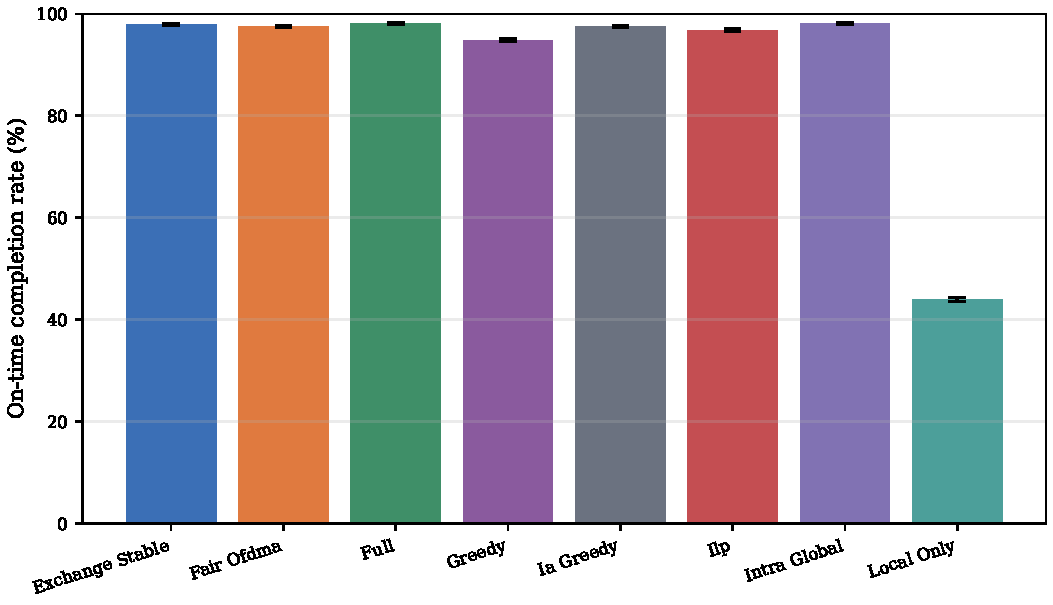
\includegraphics[width=0.9\textwidth]{../figures/thesis/main_on_time.pdf}
\caption{正式主实验按时完成率与确定性 bootstrap 区间}
\end{figure}
\begin{figure}[htbp]
\centering
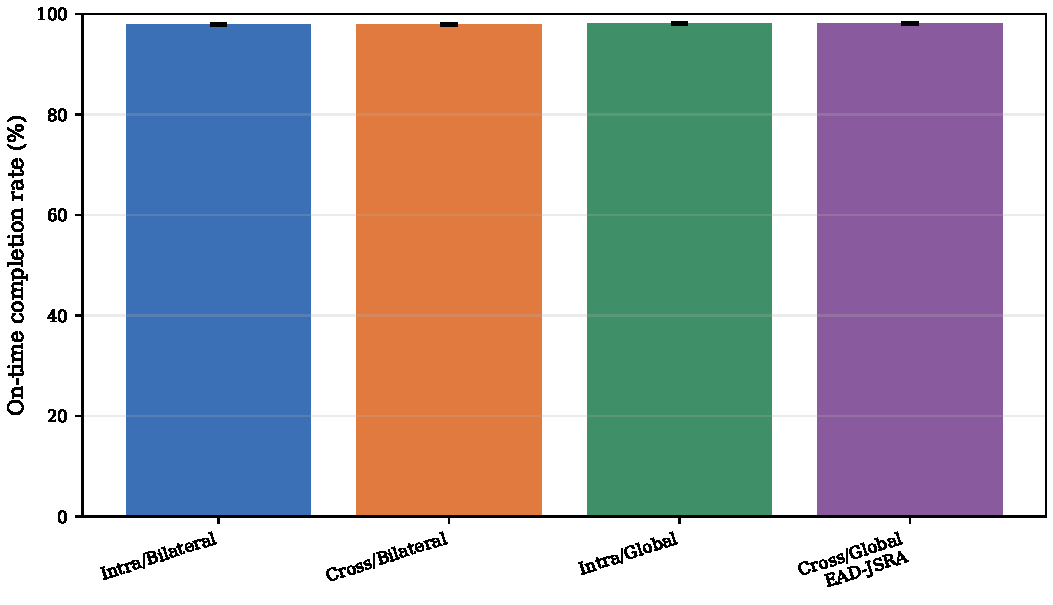
\includegraphics[width=0.78\textwidth]{../figures/thesis/pairing_ablation.pdf}
\caption{创新点一的拓扑与接受准则消融}
\end{figure}
\begin{figure}[htbp]
\centering
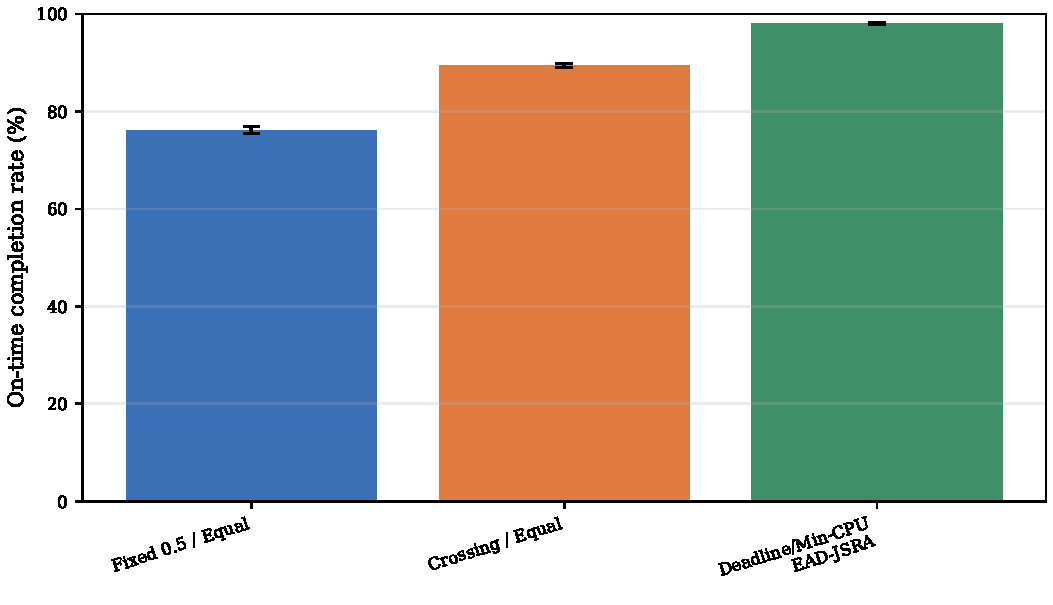
\includegraphics[width=0.78\textwidth]{../figures/thesis/resource_ablation.pdf}
\caption{创新点二的资源策略消融}
\end{figure}

\section{最优性、效率与鲁棒性}
小实例完整枚举中，启发式达到最优完成数的时隙比例为 \ExactOptimalPercent{}，平均完成数差距为 \ExactMeanCompletionGap{}；该结果仅覆盖冻结的小搜索空间。$N=20$ 的调度 P95 为 \FullRuntimePNinetyFiveMs{} ms。最终调度 SIC 违规计数为 \SICViolationCount{}。

随 $N$ 增长，所有方法按时率下降，full 在 $N=10\ldots50$ 均略高于 exchange-stable；随 $K$ 增长性能趋于饱和。$K=1$ 时 full 略低于 exchange-stable，$K=5$ 时二者持平，故不作全范围严格占优主张。轻负载下三方法均达到 100\%，重负载下 full 仍保持相对优势。

\begin{table}[htbp]
\centering
\caption{正式配对统计与主工程指标}
\resizebox{\textwidth}{!}{\begin{tabular}{lrrrr}
\toprule
Comparison & $\Delta$ (pp) & 95\% CI & $p_{\mathrm{Holm}}$ & $r_{rb}$ \\
\midrule
baseline\_exchange & 0.19 & [0.13, 0.26] & $<0.0001$ & 0.869 \\
baseline\_greedy & 3.24 & [2.96, 3.52] & $<0.0001$ & 1.000 \\
baseline\_ia\_greedy & 0.49 & [0.40, 0.59] & $<0.0001$ & 0.984 \\
baseline\_ilp & 1.30 & [1.16, 1.43] & $<0.0001$ & 1.000 \\
baseline\_ofdma & 0.58 & [0.45, 0.72] & $<0.0001$ & 0.950 \\
innovation1\_acceptance & 0.12 & [0.07, 0.16] & 0.0004 & 0.709 \\
innovation1\_cross & 0.05 & [0.01, 0.08] & 0.0201 & 0.521 \\
innovation2\_deadline & 8.69 & [8.37, 9.01] & $<0.0001$ & 1.000 \\
resource\_fixed\_half & 21.97 & [21.36, 22.60] & $<0.0001$ & 1.000 \\
\bottomrule
\end{tabular}

\bigskip

\begin{tabular}{lrrrrrr}
\toprule
Method & On-time (\%) & Drop (\%) & Delay (s) & Jain & CPU (\%) & P95 (ms) \\
\midrule
exchange\_stable & 97.91 & 2.09 & 0.6841 & 0.9993 & 33.58 & 30.14 \\
fair\_ofdma & 97.52 & 2.48 & 0.6837 & 0.9986 & 31.61 & 0.63 \\
full & 98.11 & 1.89 & 0.6843 & 0.9994 & 34.33 & 40.93 \\
greedy & 94.86 & 5.14 & 0.6804 & 0.9937 & 32.41 & 0.82 \\
ia\_greedy & 97.61 & 2.39 & 0.6838 & 0.9991 & 36.61 & 10.40 \\
ilp & 96.81 & 3.19 & 0.6828 & 0.9984 & 32.20 & 24.26 \\
intra\_global & 98.06 & 1.94 & 0.6843 & 0.9994 & 33.88 & 32.53 \\
local\_only & 43.94 & 56.06 & 0.5417 & 0.9707 & 0.00 & 0.19 \\
\bottomrule
\end{tabular}
}
\end{table}

\chapter{工程部署与研究局限}
\section{集中式控制流程}
部署时，各 UAV 在时隙开始上报候选用户、任务元数据和估计 CSI；控制器构造初始化、扫描邻域、计算 deadline/min-CPU 准入，随后下发实际服务 UAV、子载波、角色、卸载比例和 CPU。若初始化求解、结构验证或硬 SIC 检查失败，控制器应回退到已验证的可行调度，而不是发布部分结果。

\section{协调与计算开销}
全局候选评价需要跨 UAV CSI 和同频占用信息。随着用户数增大，候选扫描时间明显上升；$N=50$ 的离线扩展性实验用于暴露这一趋势。可部署版本可先用干扰上界筛除候选，再对少量候选执行完整评价，但筛选规则必须保持主目标可审计。

\section{不完美信息}
正式鲁棒性套件分别改变 CSI 误差、SIC 残差、噪声和门限。规划 CSI 与真实 CSI 分离，最终 SIC 失败记为 outage，失败传输仍保留在其他链路干扰中。该模型未覆盖高速信道老化、同步误差和控制报文丢失。

\section{外部效度}
本文使用参数化 Monte Carlo 仿真，没有声称现场部署验证。公开车辆轨迹与地面行人终端场景不一致，因此未为了增加数据集而强行接入。后续可使用带步行标签的实测轨迹替代随机游走，但仍需解释多用户组合、服务区平移和任务生成假设。

\section{未优化变量}
无人机轨迹、发射功率、电池、长期任务队列、用户优先级和跨 UAV 任务迁移均未联合优化。深度强化学习代码属于历史探索范围，不作为本文核心基线。上述限制避免把一个时隙级组合调度器包装为完整自主空中网络。

\chapter{总结与展望}
\section{工作总结}
本文针对全频复用多 UAV 分组 NOMA-MEC 时隙调度完成两项工作。第一项通过显式实际服务 UAV、Replace/Position/CrossUAV 邻域和全局严格改进，内部化跨无人机干扰外部性。第二项由截止时间推导最小卸载比例和最小 MEC CPU，并以排序前缀实现最大任务数准入。

正式 \ConfirmatorySeedCount{} 种子实验中，完整方法达到 \FullOnTimePercent{}；创新点一的 CrossUAV 独立贡献为 \InnovationOneCrossGainPP{} 个百分点，全局接受贡献为 \InnovationOneAcceptanceGainPP{} 个百分点；创新点二贡献为 \InnovationTwoGainPP{} 个百分点。完整小实例枚举匹配比例为 \ExactOptimalPercent{}，最终 SIC 违规为 \SICViolationCount{}，$N=20$ 调度 P95 为 \FullRuntimePNinetyFiveMs{} ms。

\section{结论边界}
创新点一是在高完成率强基线上的稳定小增量，创新点二具有更明显的工程效果。论文不把轨迹、功率、深度强化学习或一般复杂性结论作为额外创新，也不声称在所有 UAV 数量和负载下严格占优。

\section{后续工作}
后续可研究分布式候选筛选、真实步行轨迹驱动验证、信道老化下的稳健调度、带权任务准入及轨迹/功率联合控制。任何扩展均应保持唯一任务语义、同轨迹公平比较和可校验产物链。

\backmatter
\bibliographystyle{plainnat}
\bibliography{../paper/refs_v2}
\end{document}
